\chapter{Background: User Steering in Large-scale Workflows in CSE}
\label{chap2}


In this chapter, we provide the background for this thesis.
We begin with a brief description on the fundamental concepts
of the background (Sec. \ref{chap2_sec_basic_concepts}),
then we present a dataflow-oriented approach that gives
the basis for this thesis (Sec. \ref{subsec_datacentric}),
afterward, we describe CSE applications' characteristics in detail and showing real-world cases (Sec. \ref{sec_cse_apps}), then we present how the background work
has used data management techniques to support CSE experiments (Sec. \ref{section_workflow_steering_db}), and finally conclude with W3C PROV standard data representation for provenance (Sec. \ref{sub_w3cprov}).


\section{Basic Concepts and Terminology}
\label{chap2_sec_basic_concepts}

This section briefly describes the basic concepts and terminology used in this thesis. The goal of this section is to provide a glossary with informal definitions for the fundamental concepts. Formal definitions and more detailed descriptions with rich examples are presented in the following sections and chapters.

\subsubsection{Workflow}

CSE experiments are characterized by the execution of one or more CSE applications, which are software that implement complex algorithms and process large volumes of scientific data in large-scale computers \cite{Rude2016Research}.
These CSE applications can be modeled using a \textit{scientific workflow} (also known as \textit{large-scale workflow} or \textit{workflow}, for short) abstraction
\cite{Bernholdt2017Improving, Bauer2016In, F.daSilva2017characterization}.
Modeling CSE applications as workflows contributes to the overall CSE experiment because it makes the workflow data explicit, which need 
to be analyzed and potentially adapted.
In this thesis, we use the term \textit{workflow} as an abstract concept that means a composition of pieces interconnected through data. In traditional workflow literature, these pieces are usually called \textit{workflow activities}, or \textit{activities} for short  
When concretized, an activity can be either a black-box program, program functions, methods, or blocks of code in a script, depending on the CSE applications being modeled as a workflow \cite{F.daSilva2017characterization, Silva2017Raw, Souza2017Data, Ikeda2013Logical}.

\subsubsection{The Two Ways CSE Users Conduct their Experiments: Workflow Scripts and WMSs}

In this thesis, we consider the two typical ways that CSE users conduct their experiments on large-scale computers.

\crossref{V6: fez falta usar artigos clássicos para referendar diversas afirmações}
One way is by developing \textit{parallel CSE workflow scripts}, or \textit{workflow scripts} for short. These scripts execute a sequence of computing commands that typically invoke highly parallel libraries for data processing or performing complex computations \cite{Bernholdt2017Improving, Bauer2016In}.

The other way is by using \textit{WMSs}, like Chiron \cite{Ogasawara2011algebraic}, Kepler \cite{Nguyen2015WorkWays:}, and Pegasus \cite{Deelman2015Pegasus}.
Differently than the previous way, where CSE users write their own scripts to control the parallelism of their applications, when using a WMS, users typically rely on it to manage the parallel execution of their applications. Cases for WMSs are executions of scientific software that process the same computation over large datasets in parallel, commonly searching for a solution in a large solution space, as a parameter sweep in an embarrassingly parallel execution exploiting data parallelism
\cite{F.daSilva2017characterization, Silva2017Raw, Souza2017Data}.

\subsubsection{Workflow Data and Dataflow}

When modeling the workflows, the CSE users specify the \textit{workflow data}, which are the data processed (\ie{} consumed and generated) during the workflow execution, like scientific data files and parameters for the algorithms or numerical methods.

The workflow data are organized as \textit{datasets} and the activities operate over the data to \textit{transform} them. Thus, in a workflow execution, \textit{input datasets} are consumed by \textit{data transformations} that produce \textit{output datasets}, which can be consumed by subsequent data transformations, forming a \textit{dataflow}
\cite{Silva2017Raw, Souza2017Data}
.


\subsubsection{User Steering}

\textit{User steering} (also known as \textit{computational steering}) is a concept that means that users are enabled to interactively and dynamically drive a computational process while it is still running (\ie{} online, at runtime, during execution).

In workflows, \textit{workflow steering} is the ability that allows users to interactively analyze (\eg{} inspect, visualize, monitor) or adapt (\eg{} tune parameters, change input datasets) the workflow data online \cite{Mattoso2015Dynamic}.

\textit{To steer a workflow} is the action of performing workflow steering.

\textit{Steering actions}
are the individual user interactions performed during workflow steering, like asking a monitoring query (in case of \textit{online data analysis}) or tuning a parameter (in case of \textit{online data adaptation}).

When users steer, they generate \textit{user steering action data}, which are important information that helps to understand the steering actions and their influence on the workflow data. They consist of data informing: \textit{when} the action happened, \textit{why} the user decided to act, \textit{how} the action occurred, \textit{which} workflow data were analyzed or adapted, \textit{what} was happening before and after the action, \textit{who} acted, and the type of the action itself.

The \textit{track of steering actions} is a historical record containing important information that allows understanding the steering actions and their influence on the workflow data. In other words, it is the steering action data properly related to the rest of the workflow data.

\textit{To track a steering action}
is to query (or analyze) its track, \ie{} its historical record.

To \textit{allow for tracking steering actions}, one needs to \textit{manage steering action data}, which means \textit{to capture the steering action data, explicitly relate them to the workflow data, and store in a database ready for online queries.}


\subsubsection{Provenance Data}

Data provenance (\ie{} data lineage) contains a structured record of the data derivation process \cite{herschel_survey_2017}. It is a natural way to represent a track. In workflows, the provenance data contain not only provenance information about the data items consumed and produced, with their data derivation paths, but also data about the computational processes and agents (\eg{} users and software) involved in the workflow execution \cite{Costa2013Capturing}.
Provenance data helps to explain which and how processes were utilized to derive
each data value, in varying granularities.
Provenance data provide for data analysis,
result quality assessment, data authorship, reliability, and reproducibility of the experimental results \cite{Freire2008Provenance,Davidson2008Provenance,herschel_survey_2017}.
Such
features are considered as important as the scientific achievement or the business value
itself, since the CSE experiment's reliability can be compromised without provenance
\cite{Freire2008Provenance}. In this thesis, we leverage provenance
data management techniques to allow for tracking steering actions.

One can further subclassify workflow provenance data into \textit{prospective} and \textit{retrospective provenance data} \cite{herschel_survey_2017,Freire2008Provenance}.
Prospective provenance data provide the specification (\ie{} the definition, the structure) of the workflow, with its composing activities and possible data derivation paths.
Retrospective provenance data provide the provenance information of the data values that have been consumed or generated during the workflow execution, together with metadata about the computational processes that consumed or generated them.
In summary, prospective provenance informs what should happen when the workflow executes, whereas retrospective provenance informs what  happened when the workflow executed.
In past work, prospective and retrospective provenance data combined have been explored to deliver insightful data analyses to scientists
and users from a wide variety of scientific domains \cite{DeOliveira2015How,Souza2015Monitoramento,Silva2017Raw,Souza2017Data,silva_adding_2018,barbosa2016applying}.


\section{A Dataflow-oriented Approach for Workflows} \label{subsec_datacentric}

Data management in workflows is critical due to the inherent complexity of
the scientific domain data and the HPC requirements, \eg{}
the exploitation of data parallelism.
For steering, it is essential because it makes explicit the workflow data, which need to be analyzed and steered by the CSE users.
In this section, we provide the theoretical background for a ``dataflow-oriented approach for workflows''.
It has been been proposed by \citet{Silva2017Raw}, influenced by \citet{Ikeda2013Logical} and \citet{Ogasawara2011algebraic},
and has been refined and extended in the publications that compose this thesis.
It gives the theoretical foundation for this thesis and is the basis for the formal definition of \textit{``user steering action''}, to be defined in the following chapters.

The dataflow-oriented approach provides constructs whose essence is to promote to first-class-citizens
the elements of data flowing throughout the
activities, as opposed to an approach centered on the parallel execution control.
Following this approach, activities are called \textit{data transformations} that compose the \textit{dataflow} in a workflow, so that the dataflow is the main conceptual artifact to be managed, as opposed to the parallel execution control, which is typically managed in WMSs.
In this approach, the workflow data, consumed and generated by the data transformations, are organized as datasets, such as large data files or large matrices or mashes.
In terms of the dataflow-oriented approach, the term \textit{dataset} has slightly different semantics: it is a logical representation, concretized as a data view composed of metadata or scalar data values, of the physical datasets processed by the transformations.
This data view contains only representative data, which can potentially improve the overall data analysis of the workflow data \cite{Silva2017Raw, souza_keeping_2019}.
For instance, if a certain data transformation consumes a large matrix as a physical dataset, one could extract only representative metadata about this large matrix, its shape, and a reference pointer to the physical dataset (\eg{} a file path to where this matrix is stored in the file system). These metadata would compose the logical dataset of the physical dataset. From now on, if not explicitly distinguished, the term dataset is used as a logical dataset, with references to the physical dataset processed by the data transformation.
In this section, we precisely define these concepts.

\begin{mydef}{def:dataset}{Dataset, Data Elements, and Data Values}
A dataset $DS$ is composed of data elements, \ie{} $DS=\{e_1,...,e_m\}$.
Each data element $e_i$, $1 \leq i \leq m$, is composed of data values, \ie{} $e_i=\{v_1,...,v_u\}$.
Datasets are further specialized into \textit{Input Datasets} ($I_{DS}$) and \textit{Output Datasets} ($O_{DS}$).
\end{mydef}

\begin{mydef}{def:schema}{Data schema and attributes}
Data elements in a dataset $DS$ have a data schema $\mathbb{S}(DS) = \{a_1,...,a_u\}$,
where each element data value $v_j$  is associated with an attribute $a_j$, $1 \leq j \leq u $.
Thus, a data element can also be represented as a set of ordered pairs $\{(attribute,value)\}$, s.t.,
$e_i = \{(a_1,v_1),..., (a_u,v_u)\}$.
Moreover, attributes have a data type (\eg{} numeric, textual, array).
\end{mydef}

\begin{mydef}{def:dt}{Data Transformation}
A data transformation is characterized by the consumption of one or more input datasets $I_{DS}$ and the production of one or more output datasets $O_{DS}$.
%transforming the data following a parameterization $P$, where $P$ is a set of ordered pairs $\{(parameter,value)\}$, represented like a data element: $P = \{(p_1, v_1), ..., (p_u, v_u)\}$.
A data transformation is represented by $DT$, where $O_{DS} \leftarrow DT(I_{DS})$.
\end{mydef}

\begin{mydef}{def:derivation}{Data Derivation Path}
Let $DT_\alpha$ and $DT_\beta$ be data transformations and let $E \subset DS$ be a set of data elements produced in an output dataset $DS$ generated by $DT_\alpha$. If $DT_\beta$  consumes the elements $E$, then $DS$ is also an input dataset of $DT_\beta$. This defines a data derivation path between $DT_\alpha$ and $DT_\beta$ through
$E$, represented as $\varphi=(E,DT_\alpha,DT_\beta)$.
\end{mydef}

\begin{mydef}{def:dataflow}{Dataflow}
A dataflow is represented by $Df=(T,D,\Phi)$, where $T$ is the set of data transformations participating in the dataflow, $D$ is the set of datasets consumed or produced by the data transformations in $T$, and $\Phi$ is the set of data derivation paths between the data transformations in $T$ (adapted from background work \cite{souza_keeping_2019, Silva2017Raw, Ikeda2013Logical}).
\end{mydef}

\begin{figure}[H]
    \centering
    \includegraphics[width=\textwidth,keepaspectratio]{img/dataflow-example.pdf}
    \caption{Data derivation paths between data transformations.}
    \label{fig:derivation_paths}
\end{figure}

\noindent Figure \ref{fig:derivation_paths} illustrates these basic concepts, with two chained data transformations, $DT_1$ and $DT_2$, with a data derivation path between them through data elemets of the dataset $I_{DS2}$, which is both an output dataset for $DT_1$ and an input dataset for $DT_2$.

\begin{mydef}{def:semantics_attributes}{Semantics of attributes}
Each attribute $a_i \in \mathbb{S}(DS)$ is grouped according its semantics
$\Sigma(DS)$, s.t.:

$$\Sigma(I_{DS}) = \{F_I, V_I, P_I, L_I\} \text{ and} $$
$$\Sigma(O_{DS}) = \{F_O, V_O, C_O, L_O\}$$
where:
\begin{itemize}
\setlength\itemsep{-2mm}
\item[-] \noindent
  $F_I$ and $F_O$ contain attributes that represent pointers to
  input and output files, respectively;
\item[-] \noindent
  $V_I$ and $V_O$ contain attributes for extracted
  data or metadata from input and output files, respectively;
\item[-] \noindent
  $P_I$ contains attributes for general purpose input parameter
  values of the data transformation;
\item[-] \noindent
  $L_I$ contains attributes used by an iteration loop, \emph{i.e.},
  used for data transformations that evaluate a loop;
\item[-] \noindent
  $L_O$ contains attributes for output values especially related to an iteration
  in case of data transformations that evaluate a loop; and
\item[-] \noindent
  $C_O$ contains attributes for any output values that are explicit
  data transformation results.
\end{itemize}

\end{mydef}

Such added semantics improves the data modeling of the dataflow and
allows specifying which attributes of a dataset are parameters to
be steered. For example, attributes that represent parameters of data transformations, like
parameters of a numerical solver, filter thresholds, ranges, have the semantics $P_I$ and are often the main target of fine tunings.

Attributes with $F_I$ and $F_O$ semantics represent references to large raw (textual, imagery, matrices,
binary data) scientific data files in a wide variety of formats
depending on the scientific domain (\eg{} FITS for astronomy,
SEG-Y for seismic, NetCDF for \myabbrev{CFD}{Computational Fluid Dynamics} simulations).

$V_I$ and $V_O$ contain representative data (often scalar values or metadata) that compose the views over the large raw data files. They facilitate users to have a big picture of the content of
the files through them.

Besides large scientific data files produced by data transformations,
they may produce explicit output results, represented using the $C_{O}$ semantics. They are scalar values
or small arrays that are meaningful for the overall result data analysis. Examples are QoIs, like errors, convergence, and accuracy;

In data transformations that
evaluate loops, each iteration may be modeled as a loop evaluation
execution, like $while \ i \ < MAX$.
Examples of attributes with semantics $L_I$ are loop-stop
conditions (\eg{} $MAX$ in the case loops if the form of $while \ i < MAX$ or $threshold$ in case of loops in the form of $while \ error > threshold$).
Examples of $L_{O}$ are attributes that contain the
current values being used to evaluate a loop, which are updated at each
iteration (\eg{} $i$ and $MAX$).
Moreover, the semantics of a dataset $DS$ may not apply
to all attributes. For example, if a data transformation does not
evaluate a loop, the semantics $\Sigma(DS)$ of the datasets processed by this data transformation do not
contain $L_I$ or $L_O$.


\section{CSE Applications}
\label{sec_cse_apps}

As briefly described in Section \ref{chap2_sec_basic_concepts},
we consider the two typical ways that CSE users conduct their experiments on large-scale computers: one is by executing their applications as workflow scripts and the other is by
using a WMS to manage their applications. In Section \ref{subsec_scripts}, we provide details for workflow scripts illustrating examples of real-world applications that we use as use cases for our experiments; Section \ref{subsec_blackbox}, for applications for WMSs; and in Section \ref{cse_users} we characterize the
 scientists and engineers involved in CSE.

\subsection{CSE Applications in Workflow Scripts}
\label{subsec_scripts}

Writing and executing CSE applications in workflow scripts is one of the two typical ways CSE users automate the execution of their CSE experiments in large-scale computers.
This way is typically followed by CSE users who are experts in programming complex scientific computing tools, like numerical solvers.
The notion of ``script'' used in this thesis means that it is a sequence of computational steps, developed by CSE users, which automates a batch execution of a CSE experiment on an HPC machine. These scripts can be written in a scripting language, like Python or Shell, or a compiled language.
However, as described by \citet{Silva2018Capturing}, the software ecosystem for developing these applications involves
more than writing scripts or invoking a chain of legacy scientific
codes.
CSE users develop their simulation codes based on
complex mathematical modeling that results in invoking components of CSE
frameworks and libraries. For example, components are invoked to provide
for: (i) support for partial different equation discretization methods like libMesh, FEniCS,
MOOSE, GREENS, OpenFOAM; (ii) algorithms for solving numerical
problems with parallel computations, like PETSc, LAPACK, SLEPc; (iii)
runtime visualizations, like ParaView Catalyst, VisIt, SENSEI; (iv)
parallel graph partitioning, like ParMetis, Scotch; and (v) I/O data
management like ADIOS.
More recently, we have witnessed the popularity boom of \myabbrev{ML}{Machine Learning} libraries, like TensorFlow and PyTorch, which also process data in parallel, to \eg{} train ML models and are often invoked in codes written by ML specialists.
As a result, the software code is a workflow script, meaning that to run the underlying mathematical modeling, it requires
invoking functions, components, or APIs from these libraries or
frameworks.


As opposed to the CSE applications that are good cases for WMSs (Sec. \ref{subsec_blackbox}), these workflow scripts have intrinsic parallelism, not necessarily embarrassingly, usually implemented by the CSE users.
Thus, WMSs, which are designed to control the parallel execution, cannot be adopted to manage the execution of these scripts because there will be conflicts caused by the competition for resources between the parallel programming libraries invoked by the script the WMS engine. Anyhow, these CSE users still need provenance data management.

Despite the several solutions available for making workflow scripts
provenance-aware \cite{Stamatogiannakis2016Trade-Offs,Moreau2018Templating,Pimentel2017noWorkflow:},
capturing provenance data in these workflow scripts in CSE is still an open issue.
The challenges are mainly related to performance and provenance
granularity. Solutions that are easy to deploy collect provenance
in very fine grain and present a significant overhead, while solutions
that are based on function calls present low overhead and granularity is
controlled by the code instrumentation \cite{Stamatogiannakis2016Trade-Offs}.
 One disadvantage of instrumentation is the need to have access to the code, which is not an
issue for workflow scripts as very often the code to be instrumented is written by the CSE user, who can assist in instrumenting
\cite{Silva2018Capturing}. 
In Chapter \ref{chap3}, we discuss the support for steering in scripts.
Next, we present a real case of a workflow script.


\subsubsubsection{Computational Fluid Dynamics in Geoscience: libMesh-sedimentation}
\label{sub_libmesh}

libMesh-sedimentation
\cite{Camata2018In}
is a
Computational Fluid Dynamics workflow in the Geoscience domain, used in the O\&G industry. It implements a
simulation solver built on top of a widely used parallel finite element library,
libMesh \cite{Kirk2006libMesh},
which supports parallel simulation of multiscale, multiphysics applications.
libMesh interfaces with several libraries for Computational Science and Engineering applications (\eg{} PeTSc, Metis, Parmetis, LAPACK).
Also, scientific visualization tools like ParaView \cite{Ayachit2015ParaView},
are used to help to gain insight from the computations.
The resulting application can be seen as an iterative workflow, implemented as a script.  
In applications like libMesh-sedimentation, users typically set up
the QoIs and several parameters for the numerical methods. Examples of
parameters are tolerances for linear and nonlinear solvers, number of
levels for mesh adaptation, tolerances for space and time error
estimates. These parameters have a direct influence on the accuracy
and simulation costs, and bad choices may lead to inaccuracies and even
to a simulation crash.
As an example, the number of finite elements
predicted by the mesh adaptation procedure may exceed the memory
available in a processor, and the simulation is halted with an error
message. In simulations with complex dynamics, it is often very
difficult to set-up \textit{a priori} a maximum number of finite elements per
core that will guarantee the necessary accuracy without exhausting the
available resources.
Figure \ref{fig:libmesh} shows the libMesh-sedimentation solver modeled as an iterative workflow, composed of six data transformations with a dataset between each transformation. Particularly, the \codefont{Solver} part of libMesh-sedimentation is modeled as a data transformation that evaluates a time loop.


\begin{figure}[H]
    \centering
    \includegraphics[width=\textwidth,keepaspectratio]{img/libMesh-workflow.pdf}
    \caption{libMesh-sedimentation Workflow.}
    \label{fig:libmesh}
\end{figure}




\subsection{CSE Applications in Workflow Management Systems (WMSs)}
\label{subsec_blackbox}

Using a WMS is the other way for automating the execution of CSE experiments in large-scale computers. Good cases for WMSs
comprise experiments that are characterized by the execution of a same program or chaining of programs to process a very large dataset. Usually, each individual execution of one of these programs is not parallel, so to speed up the processing of the datasets, one can exploit data parallelism on an HPC machine \cite{F.daSilva2017characterization}.
Applications with these characteristics can highly benefit from the
efficient parallel execution control provided by WMSs because since there is no parallelism within workflow activity being managed by the WMS, the competition for computing resources is significantly reduced.
Also, WMSs provide mechanisms that facilitate the modeling of the data transformations and the dataflow and many WMSs already provide provenance data management mechanisms. \cite{Mattoso2015Dynamic}.

Another characteristic is that these applications are typically black-boxes, meaning that the CSE users either do not have access to their source code or having the source code access is not relevant for the overall experiment. Also, even if they did have access to the code, these users typically do not want to rewrite complex (already tested,
optimized, and stable) scientific software.
Thus, although the input and output datasets of the data transformations are known,
the internal computation, which contains how the data are transformed, is opaque.

In Chapter \ref{chap3}, we discuss the support for workflow steering in existing WMSs. Next, we describe real-world CSE application examples that can be used within WMSs and how they can be modeled used our dataflow-oriented approach.

%\input{history/montage_and_sciphy}

\subsubsubsection{Structure Analysis: Ultra-deepwater's Risers Fatigue Analysis} \label{sub_rfa}

The Risers Fatigue Analysis is an O\&G workflow for ultra-deepwater oil production systems.
Risers are fluid conduits between subsea
equipment and the offshore oil floating production unit. They are
susceptible to a wide variation of environmental conditions
\eg{} sea currents, wind speed, ocean waves, temperature), which
may damage their structure. The fatigue analysis workflow adopts a
cumulative damage approach as part of the riser's risk assessment
procedure considering a wide combination of possible conditions. The
result is the estimate of riser's \emph{fatigue life}, which is the
length of time that the riser will safely operate. The Design Fatigue
Factor may range from 3 to 10, meaning that the riser's fatigue
life must be at least 3 to 10 (according to the factor)
 times higher than the service life
\cite{DetNorseVeritas2010Recommended}.

Sensors located at the offshore platform collect external conditions and
floating unit data, which are stored in multiple raw files. Offshore
engineers use specialized programs (mostly simulation solvers) to
consume the files, evaluate the impact of environmental loads on the
risers in the near future (\eg{} risk of fractures), and estimate
the risers' fatigue life. 
Figure \ref{fig:rfa_wf} shows the Risers Fatigue Analysis workflow, composed of seven piped programs (represented by data transformations) with a dataset in between each transformation.

\begin{figure}[H]
    \centering
    \includegraphics[width=\textwidth,keepaspectratio]{img/rfa.pdf}
    \caption{Risers Fatigue Analysis Workflow \cite{DetNorseVeritas2010Recommended}.}
    \label{fig:rfa_wf}
\end{figure}

Risers Fatigue Analysis is modeled as parameter sweep workflow, where each task of \codefont{Data Gathering} (data transformation $DT_1$) decompresses one large file
into many files containing important input data, reads the decompressed
files, and gathers specific values (environmental conditions, floating
unit movements, and other data), which are used by the following
data transformations. \codefont{Preprocessing} (data transformation $DT_2$) performs pre-calculations and
data cleansing over some other finite element mesh files that will be
processed in the following data transformations. Stress Analysis (data transformation $DT_3$) runs
a computational structural mechanics program to calculate the stress
applied to the riser. Each task consumes pre-processed meshes and other
important input data values (gathered from $DT_1$) and generates
result data files, such as histograms of stresses applied throughout the
riser (this is an output file), and stress intensity factors in the
riser and principal stress tensor components. It also calculates the
current curvature of the riser. Then, \codefont{Stress Critical Case Selection}
(data transformation $DT_4$) and \codefont{Curvature Critical Case Selection} (data transformation $DT_5$)
calculate the fatigue life of the riser based on the stresses and
curvature, respectively. These two transformations, $DT_4$ and $DT_5$, filter out results
corresponding to risers that certainly are in a good state (no critical
stress or curvature values were identified). Those cases are of no
interest to the analysis. \codefont{Calculate Fatigue Life} (data transformation $DT_6$) uses
previously calculated values to execute a standard methodology
\cite{DetNorseVeritas2010Recommended}
and calculate the final fatigue life value of a riser.
\codefont{Compress Results}
(data transformation $DT_7$) compresses output files by a riser.



\subsection{Computational Scientists and Engineers}
\label{cse_users}

This work aims at supporting one type of user, \ie{}
computational scientists and engineers,
who are the typical users of a user-steered
workflow. However, steering workflows in HPC usually
involves several users with different levels of expertise on each
of the aspects involved in the process. We consider three types of
users: domain specialist, computational scientist or engineer, and computer
scientist or engineer.

\subsubsubsection{Domain Specialists}

Examples are geologists, biologists, and
experimental physicists. They are very familiar with concepts,
nomenclature, and semantics of the domain. They are commonly very good
at understanding the scientific hypothesis, results and data
interpretation. They may not have programming or computational skills.
The resulting data of a complex computational simulation are often
delivered to them as well organized, cured, and with some aggregations,
visualizations, plots, and dashboards. Their main work is typically to
give sense to these cured data.

\subsubsubsection{Computational Scientists and Engineers}

Examples are bioinformaticians,
computational physicists, engineers, and parallel scientific application
developers. They are not domain specialists, but have knowledge in the
domain, although more focused on the computational aspects.
They typically have programming and computational skills.
They are more prone to learning
new computing technologies and use new systems that support their
computational simulations.
They know how to analyze domain-specific data and organize large raw data files into analyzed data so
they can work together with domain specialists to interpret the
data.
They know how to chain the different data transformations and
design a workflow to attend the main goal of a CSE experiment.
They can also operate WMSs or dispatch jobs in an HPC cluster.

\subsubsubsection{Computer scientists and Engineers}

They are experts in developing tools,
methods, or systems that support large-scale simulations. Examples are
HPC, data management, workflow solution specialists.
Often, computer scientists or engineers work
closely with computational scientists or engineers to obtain the best performance for
an HPC simulation and achieve the goal of the CSE experiment.
They can analyze
performance, linked with domain and provenance data to help to tune
the system, debugging, and fixing errors.



\section{Supporting Workflow Steering in CSE with Data Management Techniques}
\label{section_workflow_steering_db}

There are at least six aspects of computational steering in scientific workflows: online analysis, monitoring, adaptation, notification, interface for interaction, and computing model \cite{Mattoso2015Dynamic}. Despite the importance of them all, the first three are essential and are the ones this thesis focuses on.
Online adaptations driven by the user is at the core of user steering.
 However, users will only know how to fine-tune parameters or which subset needs further focus if they can explore partial result data during a long-lasting execution.  The \textit{workflow steering lifecycle} (Figure \ref{fig:wfsteeringlifecycle}) is therefore given by:
    (i) analyzing the workflow data online;
    (ii) choosing what, when, how to adapt; 
    (iii) adapting the workflow data online; and
    (iv) analyzing the workflow data again to investigate the consequences of the adaptation and returning to the first step until the end of the workflow execution.
 
%  \begin{enumerate}[label=(\roman*),itemsep=0pt]
%     \item Analyzing the workflow data online;
%     \item Choosing what, when, how to adapt; 
%     \item Adapting the workflow data online; and
%     \item Analyzing the workflow data again to investigate the consequences of the adaptation and returning to the first step until the end of the workflow execution.
%  \end{enumerate}

\begin{figure}[H]
    \centering
    \includegraphics[width=\textwidth,keepaspectratio]{img/wflifecycle.pdf}
    \caption{Workflow Steering Lifecycle.}
    \label{fig:wfsteeringlifecycle}
\end{figure}

In this section, we explain how users can steer the workflow based on data management techniques.
A major issue to manage data in CSE is to address the different types of data that need to be managed.
We can group the workflow data into three types: execution,
domain, and provenance, explained as follows.


\subsubsection{Managing Execution Data}

\textit{Tasks} are the basic unit of control in a workflow execution.
Lower level execution engine information, such as physical location (\ie{} virtual machine or cluster node) where a task is being executed, can highly benefit data analysis and debugging in large-scale HPC executions.
Users may want to interactively investigate how many parallel tasks each node is running.
Tasks run domain applications that can result in errors. If there are thousands of tasks in a large execution, how to determine which tasks resulted in domain application errors and what the errors were?
Furthermore, performance data analysis is very useful as users are frequently interested in knowing how long tasks are taking, how much computing resources (memory, CPU, disk IO, network throughput, etc.) are being consumed.
These workflow execution data are important to be analyzed and can deliver interesting insights when linked to domain dataflow data \cite{silva_adding_2018,Souza2015Monitoramento}.
When execution data is stored separately from domain and provenance data, these steering queries are not possible or require combining different tools and writing specific analysis programs \cite{Silva2017Raw}.
To support this, a dataflow-oriented approach allows for recording parallel workflow execution data in a way that they can be linked to domain and provenance data.

During workflow execution, typically there are many tasks to be scheduled or executed.
Considering our dataflow-oriented approach (Sec. \ref{subsec_datacentric}), for each execution of a data transformation (also known as \textit{data transformation execution}), there is a \textit{task}. Although tasks are more closely related to the execution control, there are essential metadata that should be captured and coherently related to the domain data so that the user can steer the workflow. Information such as which tasks should execute on which
computing nodes, number of tasks per node, tasks' input data, task
duration, and how much memory or computing power it consumed are
examples of execution data to be managed, which can increase the user's awareness on the CSE experiment being conducted. Execution data can be further divided into three basic categories: (i)
list of tasks to be executed along with data about them, (ii) computing
nodes to which tasks must be executed, and (iii) performance data
\cite{Ogasawara2011algebraic,Oliveira2010SciCumulus:,silva_adding_2018,Souza2015Monitoramento}. Here, we briefly describe each category:

\begin{enumerate}[label=(\roman*),itemsep=0pt]

\item \textit{List of tasks and their associated data}. This category
refers to tasks and relevant data about them. Relevant data include: domain data to be
processed by each task; status (ready for execution, running,
completed); program to be executed, its version, versioning information; command lines and arguments,
if any; and any other data that can be used to improve the steering capabilities.

\item \textit{Computing nodes that will execute the tasks.} This category refers to where each task will be executed,
\ie{} which computing node will process it. There is a list of
available computing nodes in the HPC machine with relevant data about
them. Relevant data about a computing node
include its IP address or hostname; processing capacity
\eg{} number of instructions per second); available memory; and
the total number of CPU cores. These data are useful for analyzing major execution bottlenecks associated with specific computing nodes.

\item \textit{Performance data}. This category refers to the
amount of resources each task consumed. Examples are the amount of CPU used in the task,
memory, and network; the size of files manipulated in a specific task; and
how long a task took to be completely executed. These data can be
used by monitoring and debugging tools to analyze the scientific
application's performance associated with the domain dataflow. Users can make decisions based on them.

\end{enumerate}

\subsubsection{Managing Domain Data}

The datasets that are produced and generated in the flow between data transformations are part of the domain data that compose the dataflow. To analyze intermediate data with context, the domain data must be available for steering. Keeping track of the raw data files while keeping their context and relating their content to provenance improves online data analyses \cite{Silva2017Raw}.

However, this is hard. The data size is large, as in a single file may achieve terabytes of data and there may be multiple files in a single run. The scientific data typically contain huge numerical values with dimensional data, which can be stored as large plain text files or binary formats in proprietary or domain-specific scientific file formats, such as FITS for astronomy, SEG-Y for seismic,
NetCDF for fluid simulations, or others like
HDF5.
Often, the workflows expect that those files are
stored at runtime on an HPC shared file system (\eg{} GPFS,
Lustre) for data communication between data transformations.
Capturing data references to
these large raw data files and associating the references with relevant, meaningful data values in the dataflow is a significant assist in runtime workflow data analysis
\cite{Silva2017Raw}.

\subsubsection{Managing Provenance Data}

To manage provenance data, provenance data management systems (including components of WMSs responsible for managing provenance and provenance capture tools that can be coupled to workflow scripts) capture provenance
data during workflow execution to build a workflow database.
This requires log files or other data structures. When provenance data are enriched with domain data and the
database is made user-accessible for queries, the aforementioned
analytical capabilities are highly enhanced
\cite{Ogasawara2011algebraic,Souza2015Parallel,Silva2017Raw,DeOliveira2015How}.

\subsubsection{Managing execution, domain, and provenance in a same database}
\label{subsec_wfdb}

When execution data, domain data, and provenance data are stored in the
same database at runtime, the database provides for online data analysis via monitoring, debugging, performance analysis, and interactive domain data analysis. Let us call this database as \textit{``workflow database''}. Any database is often managed
by a \myabbrev{DBMS}{Database Management System}, like MySQL, MongoDB or Neo4j. Using the Risers Fatigue Analysis workflow (Sec. \ref{sub_rfa}) as a real-world example, Figure \ref{fig:rfa_workflow_with_prov}  illustrates how the scientific domain data are managed in our dataflow-oriented approach, showing how the data elements flowing between transformations are stored as datasets linked with workflow execution data and provenance data in the workflow database.

\begin{figure}[H]
    \centering
    \includegraphics[width=\textwidth,keepaspectratio]{img/workflow-db.pdf}
    \caption{Integrating domain, execution, and provenance data in a workflow database.}
    \label{fig:rfa_workflow_with_prov}
\end{figure}

Users can analyze the data by running queries in the database query interface at any time during execution or using any application that connects to the database to plot data visualization.
To exemplify some possible interactive data analyses, Table \ref{tab:queries1} has some typical analyses that are executed for the Riser Fatigue Analysis workflow involving domain and provenance dataflow analysis. For Queries \refQ{Q1}--\refQ{Q4}, there is a history of the data elements generated in $DT_4$ and $DT_5$ since the beginning of the flow, linking each element-flow in between. For example, environmental conditions (\refQ{Q1}) and hull conditions (\refQ{Q2}) are obtained in $DT_1$, and stress- and curvature-related values are obtained in $DT_4$ and $DT_5$, respectively. To correlate output elements from $DT_4$ or $DT_5$ to output elements from $DT_1$, provenance data relationships are required. Table \ref{tab:queries2} shows interactive data analysis that integrates domain, execution, and provenance data. For such, the core idea is to relate task scheduling data with domain data at runtime and make these data available for online queries.


\begin{table}[H] 
\caption{Examples of interactive data analysis integrating domain and provenance data.}
\label{tab:queries1}
\footnotesize
\begin{tabular}{
m{.05\textwidth}
m{.87\textwidth}
}
\Xhline{4\arrayrulewidth}


\text{}\createQ{Q1}&
What is the average of the 10 environmental conditions that are leading to the largest fatigue life value?
\\ 
\hline
\text{}\createQ{Q2}&
What are the water craft’s hull conditions that are leading to risers’ curvature lower than 800?
\\
\hline
\text{}\createQ{Q3}&
What are the top 5 raw data files that contain original data that are leading to lowest fatigue life value?
\\
\hline
\text{}\createQ{Q4}&
What are the histograms and related finite element mesh files when computed fatigue life based on stress analysis is lower than 60?
\\ 

\Xhline{4\arrayrulewidth}
\end{tabular}
\end{table}


\begin{table}[H] 
\caption{Examples of interactive data analysis integrating domain, exeuction, and provenance data.}
\label{tab:queries2}
\footnotesize
\begin{tabular}{
m{.05\textwidth}
m{.87\textwidth}
}
\Xhline{4\arrayrulewidth}

\text{}\createQ{Q5}&
Determine the average of each environmental conditions (output of 
\codefont{Data Gathering} --- $DT_1$) associated to the tasks that are taking more than the double of the average execution time of \codefont{Curvature Critical Case Selection} -- $DT_5$), grouping the results by the machines (hostnames) where the tasks of $DT_5$ were executed.
\\ 
\hline
\text{}\createQ{Q6}&
Determine the finite element meshes files (output of \codefont{Preprocessing} --- $DT_2$) associated to the tasks that are finishing with error status.
\\
\hline
\text{}\createQ{Q7}&
List status information about the 5 computing nodes with the greatest number of \codefont{Preprocessing} tasks that are consuming data elements that contain wind speed values greater than 70 km/h.
\\

\Xhline{4\arrayrulewidth}
\end{tabular}
\end{table}



Without such structured query support, users need to look for files in their directories, open and analyze them, and try to do this analysis in \textit{ad-hoc} way. Frequently, they write scripts to search in these result files.
They often interrupt the execution to fine-tune input data and save execution time. This user behavior is observed not only in the O\&G domain, but also in several other domains, such as bioinformatics, computational physics, and astronomy. More examples exploring how managing domain, execution, and provenance data in a same workflow database enables powerful online data analysis in workflows are found in background work~\cite{Costa2013Capturing,DeOliveira2015How,Souza2015Monitoramento,Silva2017Raw,silva_adding_2018}.







\section{W3C PROV and its Extensions}
\label{sub_w3cprov}


To model domain, execution, provenance data in a workflow database, it is useful to follow
existing standard data diagrams to model the data entities and relationships in such a database.
A major advantage in following standards is that it enables data interchange, interoperability, and ease of communication among scientists and engineers from different communities or that use different provenance data management systems that follow the same standard.
The \myabbrev{W3C}{World Wide Web Consortium}, acknowledged for defining standards and recommendations on the web, recommends the PROV family of documents \cite{Groth2013W3C}. Particularly, the Provenance Data Model (PROV-DM) is the general entity-relationship provenance data diagram
that gives basis to other PROV documents, such as the PROV-O for ontologies and RDF data.
PROV-DM models generic concepts like agents, entities, and activities, and how they relate to each other (Figure \ref{fig:prov_dm}), which are useful concepts for the general management of provenance data.

\begin{figure}[H]
    \centering
    \includegraphics[width=\textwidth,keepaspectratio]{img/prov-dm.pdf}
    \caption{PROV-DM General Overview \cite{Groth2013W3C}.}
    \label{fig:prov_dm}
\end{figure}

To model the specific concepts for workflows, there are specializations of PROV-DM that are PROV-compliant provenance data diagrams for workflows, like the ProvONE \cite{ProvONE} and further specializations that model workflow execution data and
domain data related to provenance data,
like the PROV-Wf \cite{Costa2013Capturing} and PROV-Df \cite{Silva2017Raw}. These provenance data entity-relationship diagrams can
be implemented by systems that manage provenance data using DBMSs with various data models, varying from triple stores \cite{castro2015abordagem} to relational DBMSs \cite{DeOliveira2015How}.

To give a concrete example, d-Chiron \cite{Souza2015Parallel} is a WMS that manages provenance data in a relational database with an instantiation of PROV-Wf.
When controlling the execution of a workflow,
say the Risers Fatigue Analysis (Sec. \ref{sub_rfa}),
the WMS populates a database with a relational database schema whose excerpt is illustrated in Figure \ref{fig:prov_rfa_dataschema}.
Relations (tables) in
light gray represent domain data and those in dark gray represent both
execution and provenance data. Domain data are part of the schema used for running the workflow.
A complete instantiation of the Risers Analysis workflow in a relational database
schema used by d-Chiron WMS is available on GitHub, where we also show concrete examples of SQL queries used to steer this workflow
\cite{d-ChironGitHub}. The SQL queries are also in the Appendix \ref{sql-codes}.

\begin{figure}
    \centering
    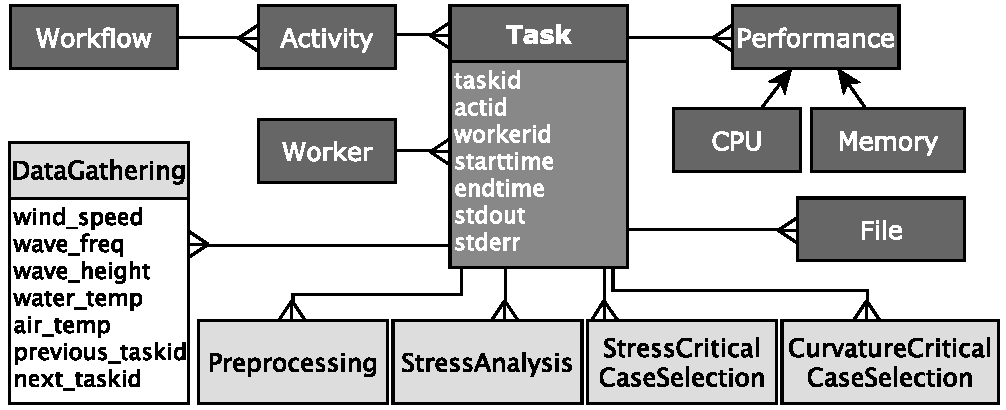
\includegraphics[width=\textwidth,keepaspectratio]{img/dchiron-data-model.pdf}
    \caption{An excerpt of a relational database schema that implements PROV-Wf.}
    \label{fig:prov_rfa_dataschema}
\end{figure}


For execution data, the main supporting relation is \codefont{Task},
which has the list of tasks to be executed and their associated data.
\codefont{Task} has a
relationship with the \codefont{Worker} relation that keeps track of which worker
(usually a computing node) executed which task.
Metadata about the files
that were processed or generated by each task execution are maintained
in the \codefont{File} relation. \codefont{Performance} relations store data about resource
consumption by each task.
Since  these data are related, a user can run analytical queries to
help users to steer the workflow
at runtime~\cite{Souza2017Data,Dias2015Data-centric,DeOliveira2015How,silva_adding_2018,Souza2015Monitoramento}. 
In this chapter, we presented the background concepts for our approach, WfSteer. In the next chapter, we survey how existing approaches support  workflow steering.
